%% Liitteiden kaavat, taulukot ja kuvat numeroidaan omana kokonaisuutenaan
%%
%% Equations, tables and figures have their own numbering in Appendices
\renewcommand{\theequation}{B\arabic{equation}}
\setcounter{equation}{0}  
\renewcommand{\thefigure}{B\arabic{figure}}
\setcounter{figure}{0}
\renewcommand{\thetable}{B\arabic{table}}
\setcounter{table}{0}

%%
%% Example of a figure, note the use of htb parameters which force
%% the figure to be inserted here
\begin{figure}[htb]
\begin{center}
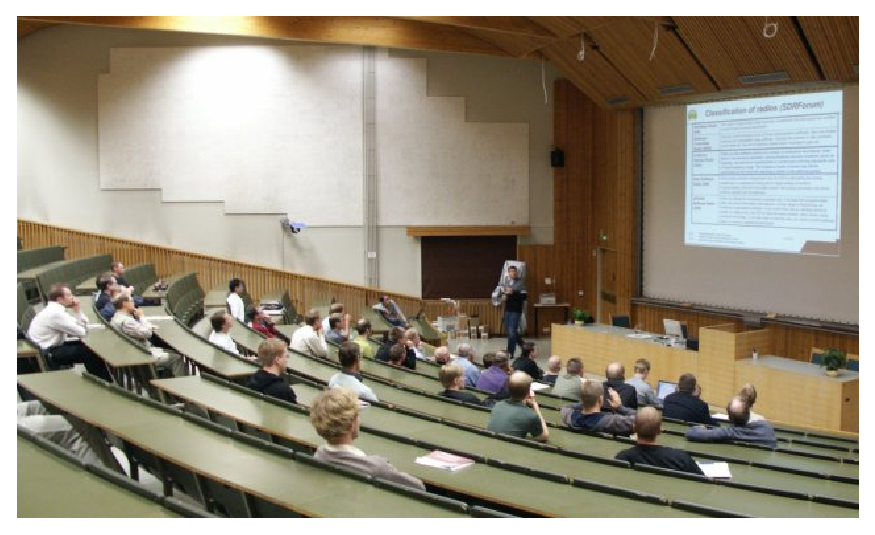
\includegraphics[height=8cm]{charts/kuva2}
\end{center}
\caption{Kuvateksti, jossa on liitteen numerointi \label{liitekuva}}
\end{figure}
%%
Liitteiden taulukoiden numerointi on kuvien ja kaavojen kaltainen:
\begin{table}[htb]
\caption{Taulukon kuvateksti. \label{liitetaulukko}}
\begin{center}
\fbox{
\begin{tabular}{lp{0.5\linewidth}}
ds
\end{tabular}}
\end{center}
\end{table}
Kaavojen numerointi muodostaa  oman kokonaisuutensa:
\begin{eqnarray}
T_{ik} &=& -p g_{ik} + w u_i u_k + \tau_{ik},  \label{liitekaava3} \\
n_i    &=& n u_i + v_i.                        \label{liitekaava4}
\end{eqnarray}